\documentclass[11pt]{article}
\usepackage{amsmath}
\usepackage{amsthm}
\usepackage{geometry}
\usepackage{verbatim}
\usepackage{graphicx}
\usepackage{amsfonts}
\usepackage{amssymb}
\geometry{bottom=2.0cm,top=2.0cm,left=2.0cm,right=2.0cm}
\begin{document}
\title{Problem Solving Homework(Week 15)}\author{161180162 Xu Zhiming}\date{\today}\maketitle
\setlength\parindent{0em}
\large\textbf{CZ: Chapter 1}\\
\normalsize
\textbf{6:}\\
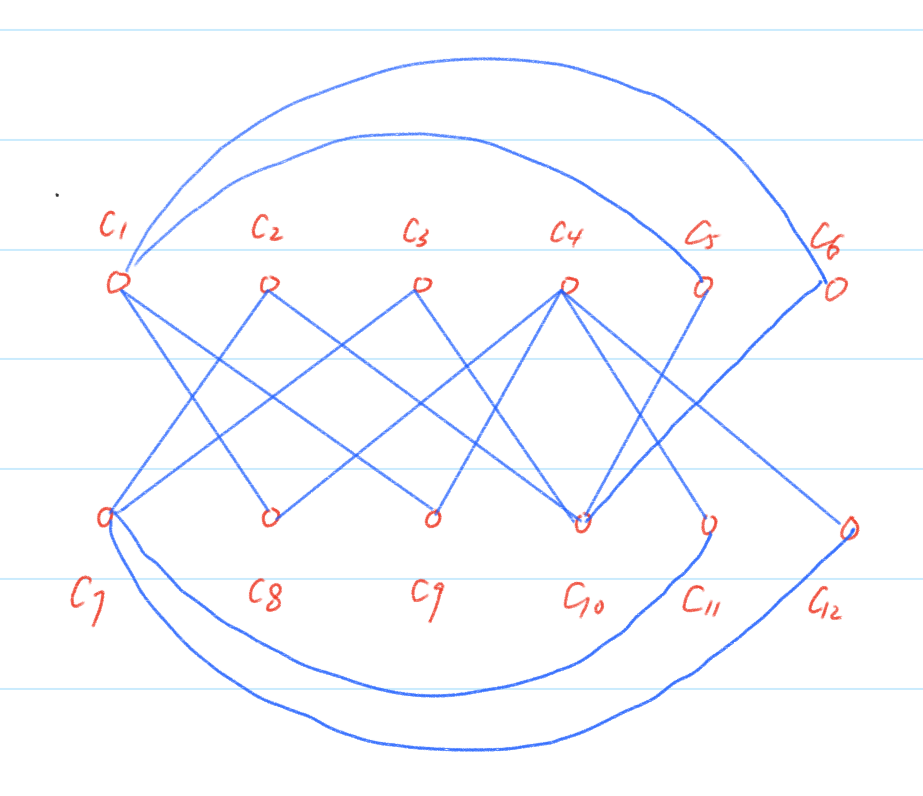
\includegraphics[scale=0.4]{1.png}\\
\textbf{8:}\\
\textbf{a.}$S_1=$\{"CAT,CET","CEA","DEA"\}    $S_2=$\{"CAT","DAT","CAU","CBT"\}    $S_3=$\{"CAT","CAU","CAV","CATS"\}
$S_4=$\{"CAT","CET","CEA","CAA"\}     $S_5$=\{"CAT","CET","CAA","CAS"\}    $S_6=$\{"CAT","DAT","EAT","FAT"\}\\
\textbf{10:}\\
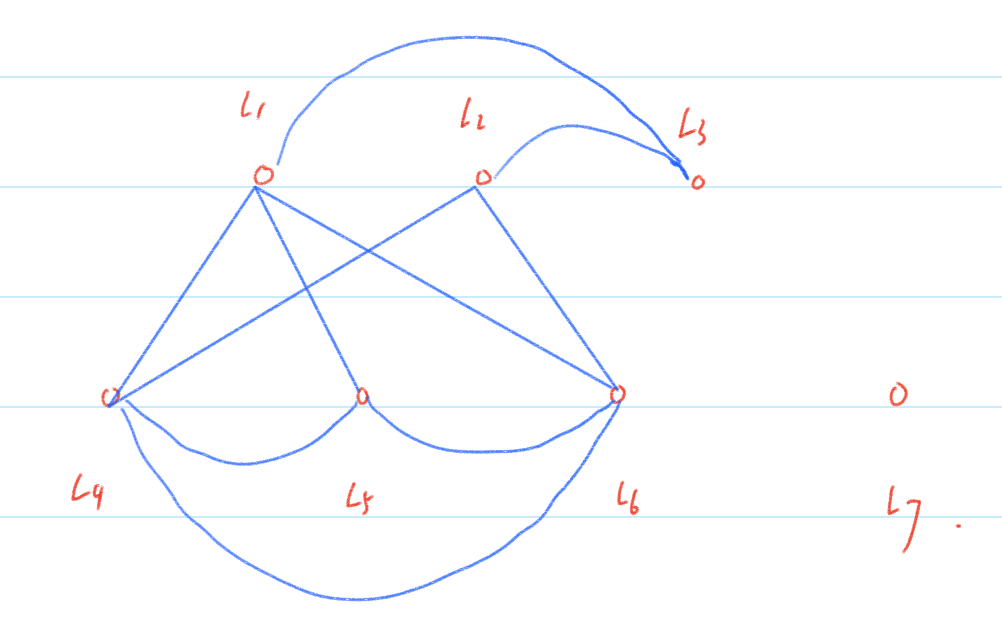
\includegraphics[scale=0.4]{2.png}\\
\textbf{14:}
\begin{proof}
We need to prove that a connected subgraph of \emph{G} that is not a subgraph proper subgraph of any other connected subgraph of \emph{G} is equal to a subgraph of \emph{G} induced by the vertices in an equivalence class resulting from the equivalence relation defined in Theorem 1.7.\\
\emph{Def.1} means that for every pair of vertices in that connected graph, say, $u$ and $v$, there exist path(s) from $u$ to $v$ and for every vertex that doesn't belong to the subgraph isn't linked with any vertex in it. \emph{Def.2} means a subgraph which is also a equivalence class by Theorem 1.7. Then for every pair of vertices in the subgraph, say, $u$ and $v$, they are connected by path(s). Besides, every vertex isn't linked to any vertex that belongs to another equivalence class.\\
Therefore, the two interpretations are equivalent.
\end{proof}
\textbf{16:}
\begin{proof}
Since $P=(u=v_0,v_1,\cdots,v_k=v),k\ge 1$ is a $u-v$ path, then $d(u,v)=d(u,v_k)=k$ and $d(u,v_i)=i$ for every $i$ with $0\le i\le k.$(From the comments under equation 1.5)  
\end{proof}
\textbf{17:}
\begin{proof}
\textbf{a.}Suppose $P$ and $Q$ have no vertices in common, namely $P=(u_0,u_1,\cdots,u_k)$,  $Q=(v_0,v_1,\cdots,v_j)$, and for every pair of $u_i(0\le i\le k)$ and $v_i(0\le i\le j)$, they are not the same. Then we can construct a walk $R=(u_0,u_1,\cdots,u_k,v_0,v_1,\cdots,v_j)$ in which no vertices are repeated. Obviously, the length of $R$ is longer than both $P$ and $Q$, which contradicts the given condition. Therefore, the assumption is wrong and $P$ and $Q$ have at least one vertex in common.\\
\textbf{b.}False, consider Figure 1.19(a) in the textbook, the diameter of this graph is 3, and both path $P'=(y,u,r,s)$ and path $P=(x,u,r,s)$'s length(=3) equals diam(H). Therefore, the statement is false.
\end{proof}
\textbf{20:}\\
\textbf{a.}Since $u$ and $v$ are vertices in a connected graph, so there exist at least a path $P=(u,x_0,\cdots,x_k,v)$. All the vertices in this path is connected, so the path is a connected subgraph of $G$. As we know, the shortest path's length is defined as $d(u,v)$, then minimum size of a connected subgraph of $G$ containing $u$ and $v$ is $d(u,v)$.\\
\textbf{b.}The order of such a subgraph is $d(u,v)+1$.\\
\textbf{22:} 
\begin{proof}
Case 1: $d_{\bar{G}}(u,v)=1$, if $u$ and $v$ is previously not adjacent in $G$, then they will be connected by an edge in $\bar{G}$, so $d_{\bar{G}}(u,v)=1$.\\
Case 2: $d_{\bar{G}}(u,v)=2$, suppose $G$ has component $A$ and $B$, $u,v\in A$. Then in $\bar{G}$, they are not connected. The shortest path from $u$ to $v$ is $P=(u,w,v)$ in which $w\in B$. So $d_{\bar{G}}=2$.\\
There is not a third case, consequently, diam$(\bar{G})\le2$.
\end{proof}
\textbf{23:}\\
\textbf{a.}
\begin{proof}%存在性证明只要找到一个就可以
Case 1$(k=1)$: For the graph $C_5=(u,v,x,y,w,u)$, $d_G(u,v)=1=d_{\bar{G}(u,v)}$.\\
Case 2$(k=2)$: For the graph $C_5=(u,x,y,v,z,u)$, $d_G(u,v)=2=d_{\bar{G}}(u,v)$.\\
\end{proof}
\textbf{b.}
\textbf{b.}Consider $P_4$, $k$ at most is 3.\\
\textbf{25:}
\begin{proof}
If $G$ isn't a bipartite, the proof is trivial. Suppose $G$ is a bipartite and it has bipartite sets including $U$ and $V$. Since $G$'s order is 5, at least one of $U$ and $V$'s order is greater than or equal to 3. Suppose $|U|=k\ge3$, then the subgraph of $\bar{G}$ induced by $U$ is the complete graph $K_k$ with $k\ge3$. Consequently, $\bar{G}$ contains a triangle, that is, there is an odd cycle in it. According to Theorem 1.12, $\bar{G}$ isn't bipartite.
\end{proof}
\textbf{30:}\\
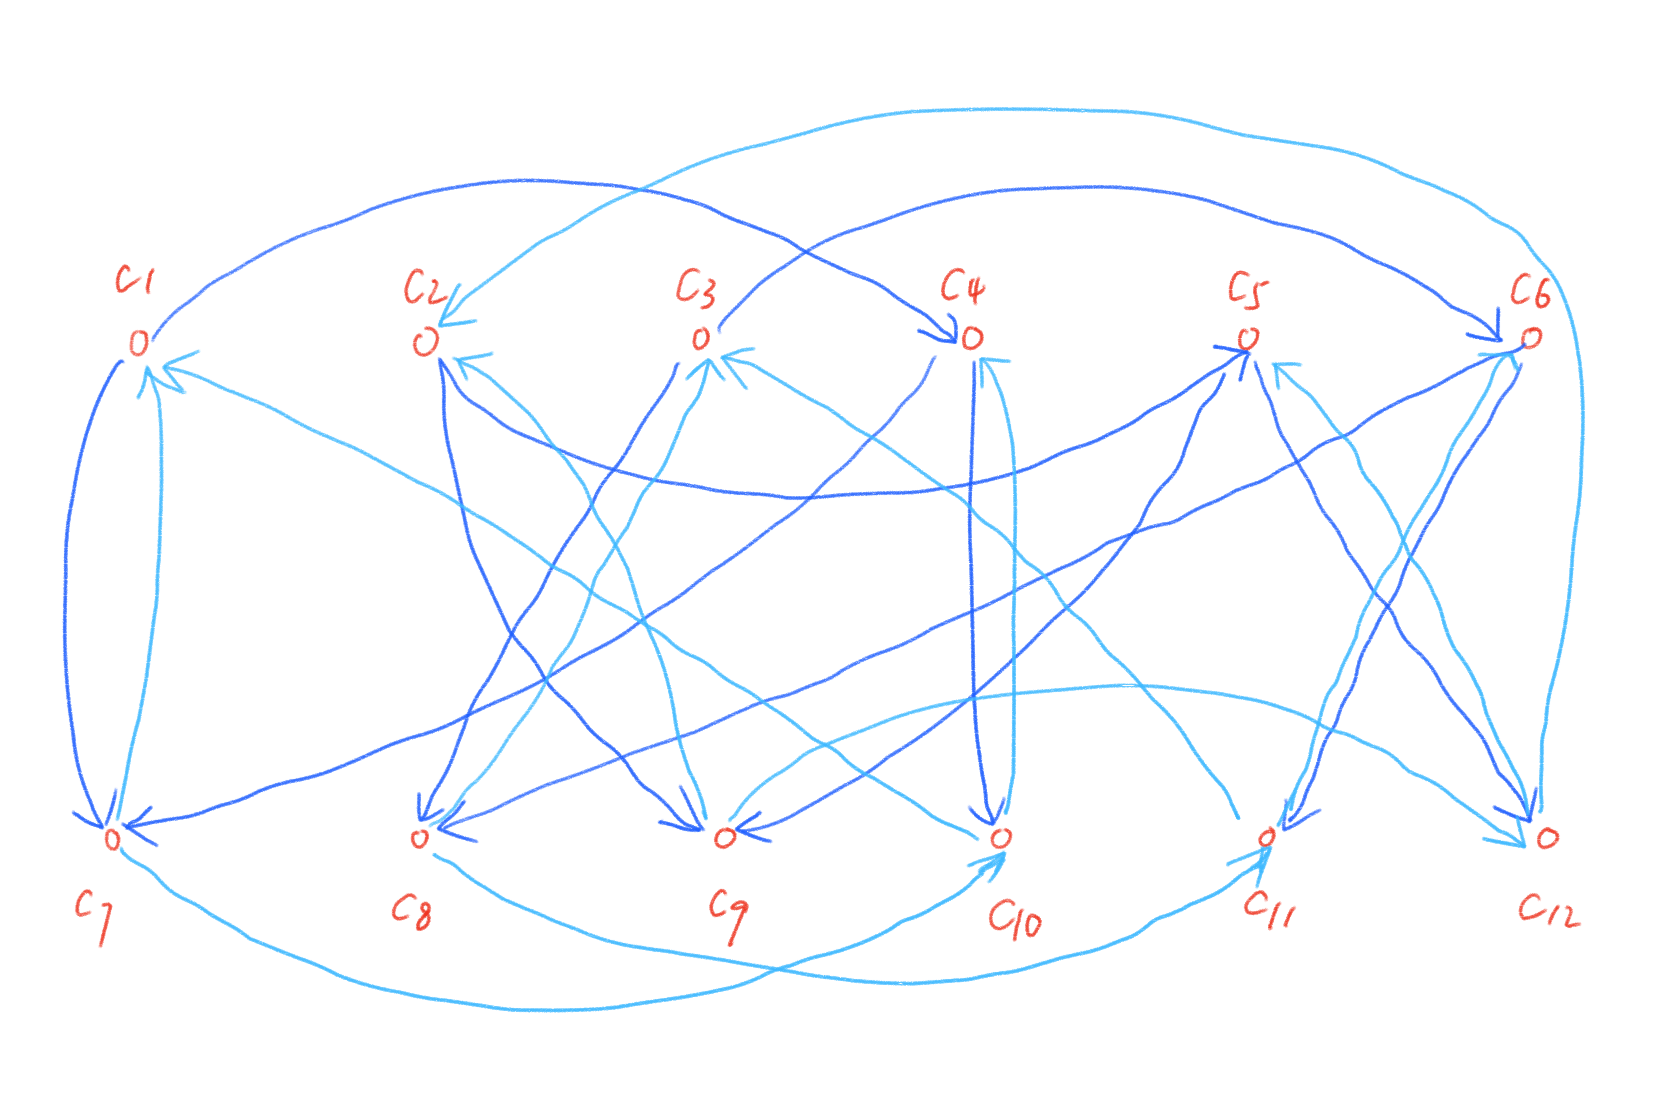
\includegraphics[scale=0.25]{3.png}\\
\textbf{31:}\\
Digraph is deifned as follows: $V(D)=\{c_1,c_2,\cdots,c_12\}$, where $(c_i,c_j)$ is a directed edge of $D$ if it is possible to obtain $c_j$ by rotating the configuration $c_i$ either $90^{\circ}$ or $180^{\circ}$ anti-clockwise about the midpoint of the checkerboard.\\
\large\textbf{CZ: Chapter 2}\\
\normalsize\textbf{6:}
\begin{proof}
By first theorem, $\sum_{v\in V(G)}deg$ $v=n(n-1)+n\cdot n+n(n+1)=3n^2$, which is twice of $G$'s size. Thus $3n^2$ is even. Then $n$ is even.
\end{proof}
\textbf{7:}\\
\textbf{a.}
\begin{proof}
Since $\sum_{u\in U}deg$ $u$+$\sum_{w\in W}deg$ $w=\sum_{v\in G}deg$ $v=2m$, so we just need ot prove that \[\sum_{u\in U}deg (u)=\sum_{w\in W}deg(w)\]We denote that $U=(u_0,u_1,\cdots,u_j)$ and $W=(w_0,w_1,\cdots,w_k)$. For each $deg$ $u_r$ and $deg$ $w_s$, the former is number of vertices adjacent to it in $W$, the latter is the number of vertices adjacent to it in $U$. As the connection between $u_r$ and $w_s$ is mutual. Each edge's two ends is some $u_r$ and $w_s$, so when calculating the degree the vertices in $U$ and $W$ are ocunted for the same time.\\
Therefore $\sum_{u\in U}deg$ $u=\sum_{w\in W}deg$ $w$, and they both equals $\frac{2m}{2}=m$.
\end{proof}
\textbf{b.}\\
Suppose the size of $G$ is $m$ and there are $x$ vertices in $W$ have degree 2.
\begin{equation*}
\begin{aligned}
deg(u)\cdot|U|&=m\\
|W|+|U|&=G.order\\
2x+4(|W|-x)&=m\\
|U|&=12\\
deg(u)&=3\\
u&\in U
\end{aligned}
\end{equation*}
Solve these equations, we obtain $x=2$, so 2 vertices in $W$ have degree 2.\\
\textbf{9:}
\begin{proof}
Suppose $V_1$ and $V_2$ are two distinct components of $G$, $v_1\in V_1$, $v_2\in V_2$ are the only two odd vertices. There are only these two odd vertices. Consider $v_1$, it is adjacent to an odd number vertices. Since these vertices are even, they are adjacent to an even number of vertices. However the remaining odd number of vertices can not satisfy this condition. Consequently, the assumption is wrong and the only two odd vertices must be in the same component.
\end{proof}
\textbf{10:}\\
\textbf{a.}\\
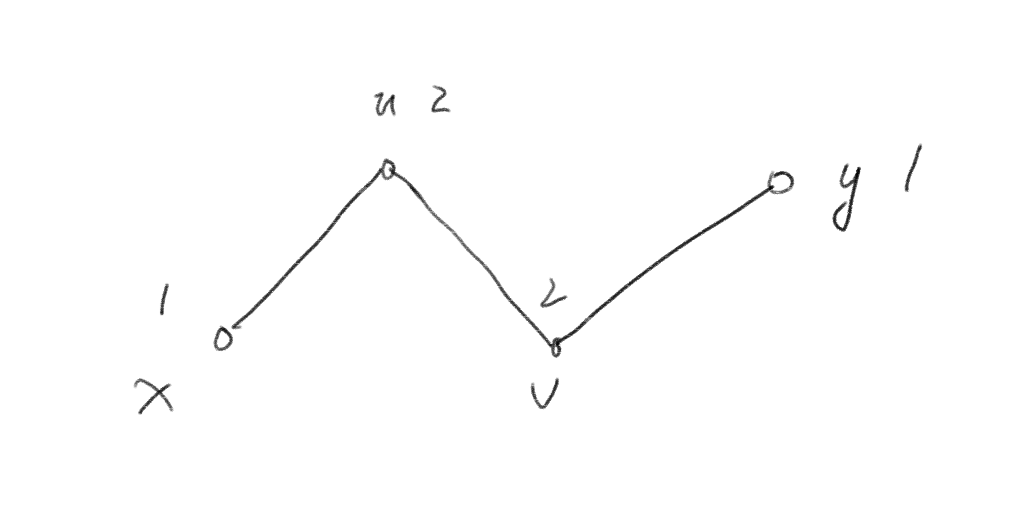
\includegraphics[scale=0.4]{4.png}\\
Consider $P_4$ in this figure, for every two nonadjacent vertices $u$ and $v$, deg $u$+deg $v\ge n-2$, and deg $x+$deg $y=n-2=2.$\\
\textbf{b.}
\begin{proof}
Suppose that a graph \emph{F} satisfying this condition has more than two components, namely, it has $k(k\ge3)$ components. Then it can be divided to \emph{k} parts, $F=(F_0\cup F_1\cup\cdots\cup F_k)$. For every pair of \emph{u} and \emph{v}, deg \emph{u}+deg \emph{v}$\le F_i.order-1+F_j.order-1(0\le i,j\le k)$. Besides, $\sum_{i=0}^{k}F_i.order=F.order$, $F_i.order(i=0,1,\cdots,k)\ge1.$ So $\exists$ deg \emph{u}+deg \emph{v}$\le n-3$, which contradicts the given condition. The assumption is wrong.
\end{proof}
\textbf{c.}Yes, the bound is sharp. Consider $2P_2\cup P_1.$\\
\textbf{13:}\\
\textbf{a.}
\begin{proof}
Suppose that it is not this case and $G$ has at least three components, $G_1$, $G_2$, and $G_3$ are part of them. Let $v_i\in V(G_i)$ for $0\le i\le 3$. Since for $v_i\ge(n-2)/3$, $G_i(1\le i\le3)$ has at least $(n-2)/3+1=(n+1)/3$ vertices. $\sum_{i=1}^{3}|V(G_i)|=(n+1)/3+(n+1)/3+(n+1)/3=n+1$, which contradicts the fact that $|V(G)|=n$. Therefore, the assumption is wrong.
\end{proof}
\textbf{b.}
\begin{proof}
Suppose that the bound is not sharp, substitute $(n-1)/3$ with $(n-1)/3-\epsilon(\epsilon\ge1)$. Repeat the calculation in \emph{a}, $\sum_{i=1}^{3}|V(G_i)|=n+1-3\epsilon\le n-2$, which can happen without contradicting the fact that $|V(G)|=n$. Consequently, the bound is sharp.
\end{proof}
\textbf{15:}
\begin{proof}
Suppose that $G$ is not a bipartite, then \emph{G} has an odd cycle \emph{C}. For two vertices $u$ and $v$ in \emph{C}, there is an even path and an odd path from $u$ to $v$, which contradicts the fact that two vertices only have an even or an odd path. So the assumption is wrong. $G$ is a bipartite. 
\end{proof}
\textbf{20:}\\
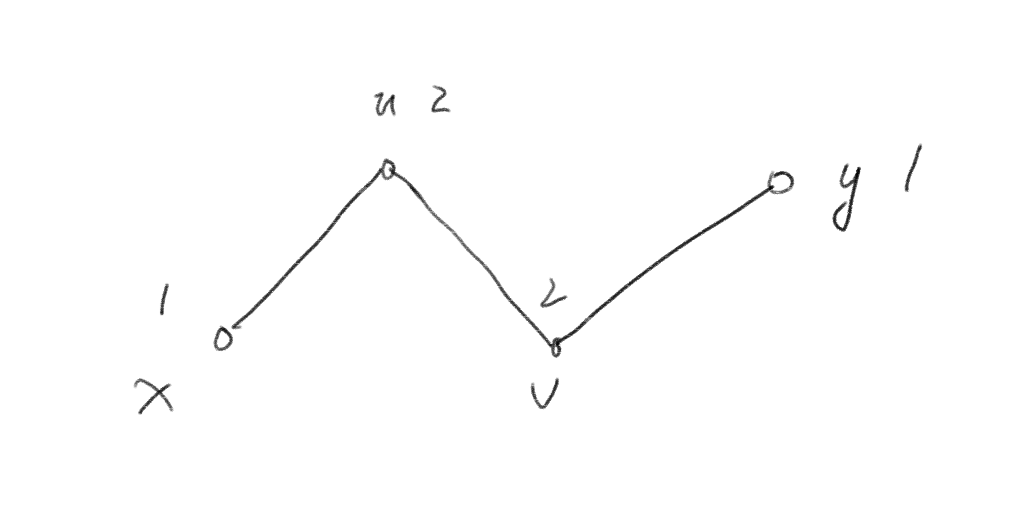
\includegraphics[scale=0.4]{4.png}\\
In this graph $P_4$, $x$ and $u$ are adjacent, but deg \emph{x}=1, deg \emph{u}=2.\\
\textbf{25:}\\
\textbf{a.}
By Corollary 2.3, $G-v$ must have an even number of vertices, so $G$ has an odd number of vertices, namely, $G$ has odd order.\\
\textbf{b.}
\begin{proof}
Suppose that $G$ does contain an odd component, then for this component $U$, $U$ is r-regular where r is odd. Besides the order of $U$ is odd, which contradicts Corollary 2.3. So $G$ does not contain any component of odd order.
\end{proof}   
\textbf{27:}
\begin{proof}
Suppose that $|U|\ne |W|$, and $|U|>|W|$. Since $G$ is an $r$-regular bipartite, then the vertices $u_i\in U$ and $w_i\in W$ all have a degree of $r$. $u_i$ is adjacent to some $w_j(1\ge j\ge|W|)$ and vice versa. Every edge connected $u_i$ and $w_j$ will increase the degree of $u_i$ and $w_j$ by 1.That's to say, since all edges are between some $u\in U$ and $w\in W$, $\sum_{u\in U}$deg $u$=$\sum_{w\in W}\in W$deg $w$. However, by our assumption, $\sum_{u\in U}$deg $u$=$r\cdot |U|<$$\sum_{w\in W}$deg $w$=$r\cdot |W|$. So the assumption is wrong. $G$'s partite sets $U$ and $W$ have the same number of vertices.
\end{proof}
\textbf{28:}\\
$G$ is r-regular and $G=H$. Or $G$ has an order of $n$, and $H$ is $K_n$\\
\large\textbf{CZ: Chapter 3}\\
\normalsize\textbf{6:}\\
Yes, because there cannot exit a one-to-one correspondence $\phi$ from $G_1$ to $G_2$.\\
\textbf{9:}\\
Not isomorphic. The two verices of degree 3 is adjacent in $G_1$ but not adjacent in $G_2$.\\
\textbf{11:}
\begin{proof}
Assume that $|U|=|W|=\alpha$. Consider a vertex in $w\in W$, deg$_G v\ge n/2$. Then deg$_{\bar{G}} v=n-1-$deg$_Gv\le n/2-1$. Besides, there are $\alpha$ vertices in $G$ that has degree geater than $n/2$. So there are $\alpha$ vertices in $G$ of degree less than $n/2$. Because there are $\alpha$ vertices in $G$ with degree less than $n/2$, there is not a vertex in $G$ with deg$_Gv=n/2$. 
\end{proof}
\textbf{13:}
\begin{proof}
The two graphs are isomorphic. By  this statement we know that the degree sequences of $G$ and $H$ are the same. Besides, since $d_G(u,v)=d_H(\phi(u),\phi(v)$, then if $u$ and $v$ are adjacent, then $\phi(u)$ and $\phi(v)$ are adjacent, vice versa. Therefore, they are isomorphic.
\end{proof}
\end{document}